% !TeX root = ../../tesi.tex

The comparative analysis of the three candidate families revealed a common trend: modern vision systems are increasingly moving beyond purely convolutional designs and are exploiting transformer-based representations in progressively more effective ways. Nevertheless, the final choice could not be based on architectural novelty alone. It had to reflect the concrete needs of the thesis, namely accurate and real-time localization of products in industrial environments, compatibility with edge-oriented deployment, and a favorable balance between predictive performance and computational cost.

Within this framework, DEIMv2 emerged as the most suitable solution. Compared with YOLOv12, it offered a more favorable overall performance--cost trade-off according to the evidence reported in the literature, combining higher detection accuracy with competitive or lower parameter and FLOP budgets in the corresponding model regimes, as illustrated in Figure~\ref{fig:DEIMvsYOLO} \cite{huang_real-time_2026,tian_yolov12_2025}. In addition, its integration of DINOv3-based representations and multi-scale adaptation made it particularly appealing for scenarios in which both local visual details and more global semantic structure may contribute to robust object detection.
Furthermore, DEIMv2's variety of model sizes and its compatibility with real-time detection requirements made it a versatile choice for the different deployment scenarios considered in the thesis, ranging from GPU-based inference to edge-oriented applications \cite{huang_real-time_2026,zhao_detrs_2024}. By contrast, part of YOLOv12's efficiency advantage depends on hardware support for FlashAttention, which is not uniformly available across all deployment environments. In this respect, DEIMv2 appears more flexible and robust as a practical choice for heterogeneous hardware settings.
\begin{figure}[h]
    \centering
    \captionsetup[subfigure]{justification=centering}
    \begin{subfigure}[t]{0.48\textwidth}
        \centering
        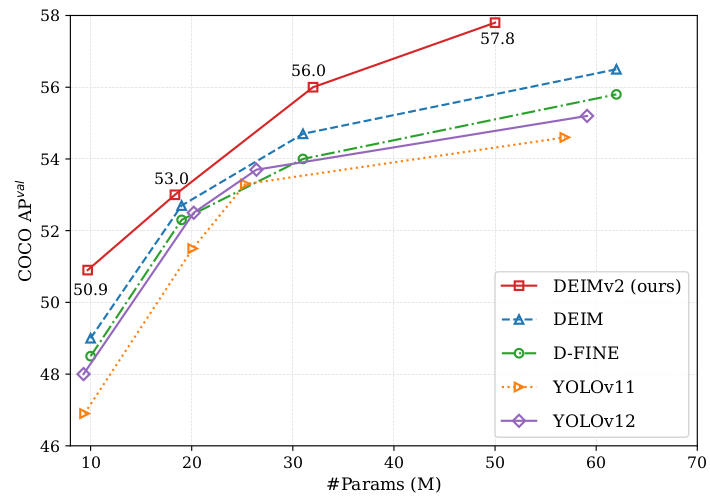
\includegraphics[width=\textwidth]{images/DEIMvsYOLO1.png}
        \caption[c]{Accuracy versus number of parameters for DEIMv2 and YOLOv12 across model scales \cite{huang_real-time_2026,tian_yolov12_2025}.}
        \label{fig:DEIMvsYOLO1}    
    \end{subfigure}\hfill
    \begin{subfigure}[t]{0.48\textwidth}
        \centering
        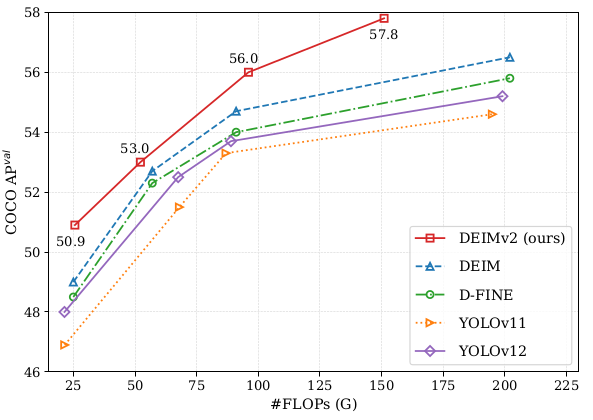
\includegraphics[width=\textwidth]{images/DEIMvsYOLO2.png}
        \caption[c]{Accuracy versus computational cost for DEIMv2 and YOLOv12 across model scales \cite{huang_real-time_2026,tian_yolov12_2025}.}
        \label{fig:DEIMvsYOLO2}
    \end{subfigure}
    \caption{Comparison between DEIMv2 and YOLOv12 in terms of accuracy, parameter count, and computational cost, highlighting the stronger overall efficiency of DEIMv2 across the considered model scales \cite{huang_real-time_2026,tian_yolov12_2025}.}
    \label{fig:DEIMvsYOLO}
\end{figure}

The comparison with EoMT requires a different interpretation, because EoMT addresses image segmentation rather than object detection. For this reason, the decisive argument was not that DEIMv2 is universally superior on a common benchmark, but that it is better aligned with the objective of the thesis. In the proposed pipeline, the essential requirement is to localize each dough ball or loaf quickly and reliably, so that subsequent modules can estimate geometric or appearance-based quantities. For this thesis, object detection is therefore the more appropriate output representation: a full segmentation model would provide richer pixel-level information, but at the cost of denser prediction, greater architectural complexity, and weaker compatibility with low-latency embedded deployment. Moreover, the advantages of EoMT are most evident when large pretrained ViTs and high-performance hardware are available, whereas the thesis prioritizes an efficient real-time detector that can be deployed in practical industrial settings \cite{kerssies_your_2025}.

For these reasons, DEIMv2 was selected as the detection model adopted in this thesis. It combines state-of-the-art real-time detection performance, strong scalability across model sizes, and a transformer-based design that remains compatible with the broader evolution of modern vision architectures. At the same time, the study of YOLOv12 and EoMT remained valuable: YOLOv12 highlighted the growing viability of attention-centric real-time detectors, while EoMT showed that large pretrained ViTs can increasingly absorb task-specific dense prediction components. Together, these works provided the conceptual background against which DEIMv2 was identified as the most appropriate choice for this thesis.
